%results
\section{Celestial Body Simulation}
Initial use of GenSequence on the planetary orbits program proved some promise in the capability of this tool. The tool generated 30 test cases. Test case 13 was programmatically named:
\vspace{1cm}

\noindent\fbox{
    \parbox{\textwidth}{
        {\fontfamily{pcr}\selectfont
        13-70-mass|right_slanted-position|right_slanted-velocity|uniform-diameter|left_slanted.csv
        }
    }
}

\vspace{1cm}
13 is the test case number and 70 is the number of rows in the test case. Each row of the file represents an instance of a planetary body. GenSequence has encoded the way each parameter was generated in the filename. So \texttt{mass|right_slanted} means that planetary masses were generated with a right slanted distribution. Position, the location of each body, was generated with a right-slanted triangular probability. The velocities of the bodies were generated uniformly. The diameters, the visible size in the program's GUI, were generated by a left-slanted distribution. The starting point of this program's test data showed this visualization:

\begin{figure}[H]
\centering
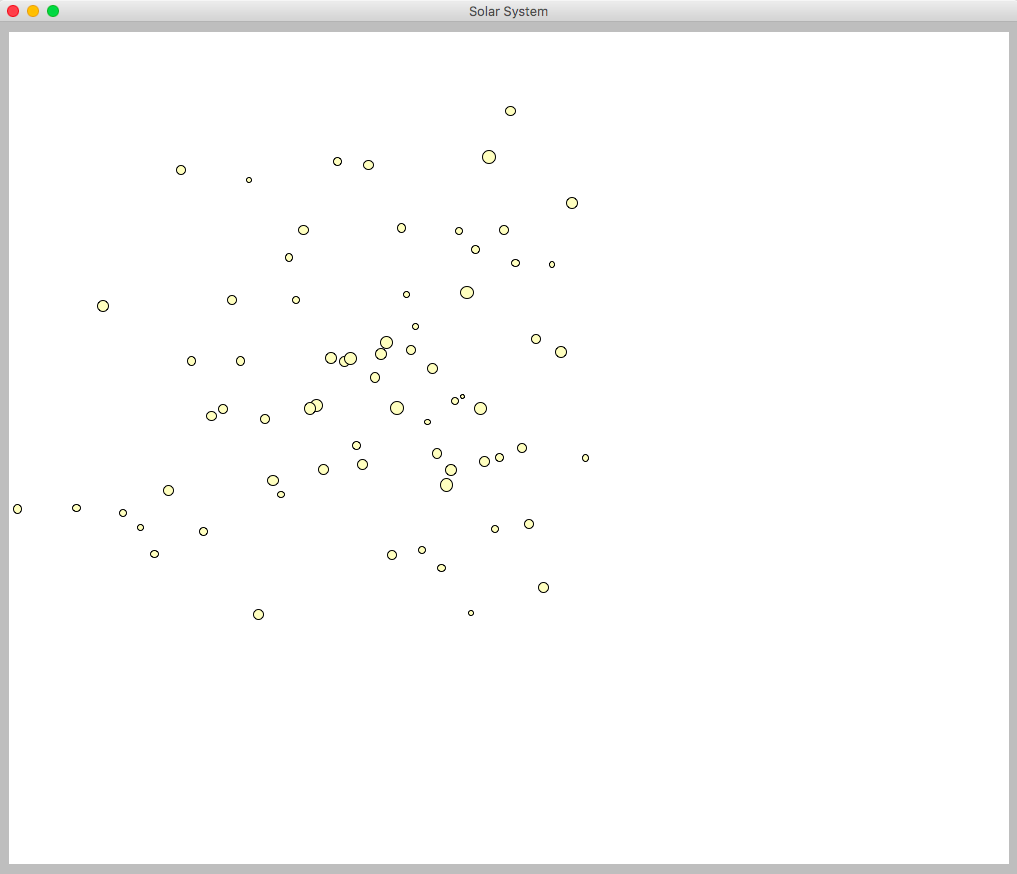
\includegraphics[scale=0.4]{start-ex.png}
\caption{Starting Locations of 70 celestial bodies}
\label{fig:startbody}
\end{figure}

Figure \ref{fig:startbody} accurately reflects the visible parameters – position and diameter. The positions were generated by a right slant and, ostensibly so, the bodies are mostly located in one region. The diameters were generated by a left-slanted distribution, clearly slanted towards a smaller diameter, with most samples appearing small or medium size, but a notable number appearing fairly large (though from the naked eye one can agree it does require close inspection).

The program tracks and draws the motion of each planetary body through time, giving a useful summary of the program's execution by the end of the simulation (665 time steps). Running test case 13 resulted in Figure \ref{fig:endbody}.

\begin{figure}[h!]
\centering
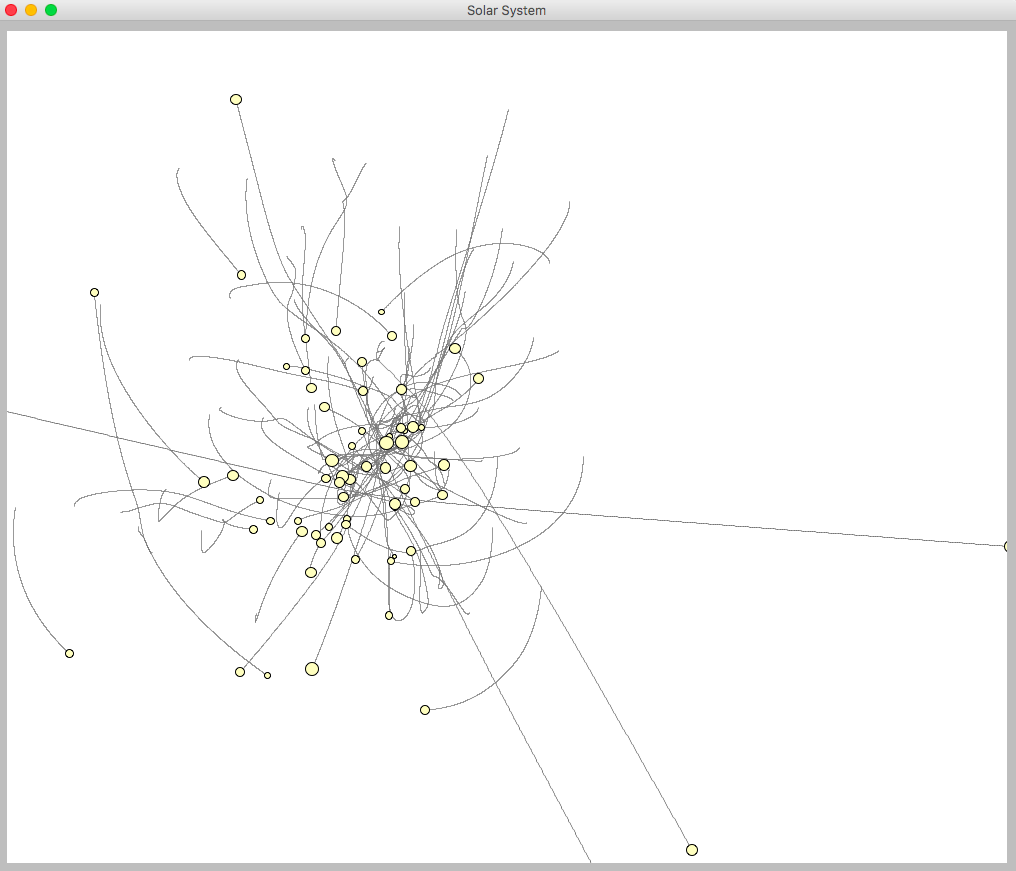
\includegraphics[scale=0.4]{final-ex.png}
\caption{Ending Locations of 70 celestial bodies after 665 time steps}
\label{fig:endbody}
\end{figure}

Spending a minute closely observing these paths registers some important observations about the natural behavior of gravity acting on planetary bodies. Some disobeyed their trajectory and were redirected by the cumulative mass in the center. The initial velocities manifested themselves as well. The paths are of all different lengths, which makes sense since they were generated by a uniform distribution.

\section{Earthquake Analysis and Visualization Program}
The earthquake analysis program performs basic statistical analysis of magnitudes, locations, and depths on a map, and also plots quake events on a map. Bigger dots represent a greater data point value (This is important to note because dots representing magnitudes describe their intensity, not their destruction coverage). One test case had a file name (test vector) of:
\vspace{1cm}

\noindent\fbox{%
    \parbox{\textwidth}{%
        {\fontfamily{pcr}\selectfont
        6-70-magnitudes|cardioid-latitudes|left_slanted-longitudes|right_slanted-depths|cardioid.csv
        }
    }%
}

\vspace{1cm}
Observing the cardioid relationship between latitudes and longitudes is confirmation of GenSequence working. GenSequence was programmed with the following information:
\vspace{1cm}

\begin{lstlisting}
#magnitudes ranges
Micro = Range(0.0, 2.0, exclusive_upper=True)
Feelable = Range(4.5, 7.9, exclusive_lower=True)
Great = Range(8.0, 9.5, exclusive_lower=True, exclusive_upper=True)
#depths ranges
Shallow = Range(0.0, 5.0, exclusive_lower=True, exclusive_upper=True)
Mid = Range(5.0, 15.0)
Deep = Range(15.0, 30.0, exclusive_lower=True)
...
# specify the relationship between magnitudes and depths
MagsDepths = Cardioid(Mags, Depths)
MagsDepths.setFavorites([(Micro,Shallow), (Great,Deep), (Feelable,Mid)])
MagsDepths.setNonFavorites([(Micro,Deep), (Great,Shallow), (Feelable,Deep), (Feelable,Shallow)])
\end{lstlisting}

\vspace{1cm}
This is the literal implementation of the tool describing the most frequently occurring data pairs in this test case. Low intensity magnitudes should be near Earth's surface (values closer to 0) and very intense magnitudes should occur deep below the earth's surface (values closer to 30). Moreover, it is not very frequent that low-intensity earthquakes occur deeply, and high-intensity earthquakes occur near the surface. \footnote{This assumption may be entirely false about the nature of earthquakes. This trend is one I invented to add functionality to GenSequence, one that could easily be reversed by any seismologist user of the program.}

The plots of magnitudes and depths (Figure \ref{fig:magsdepths}) show this constraint propagating:
\begin{figure}[H]
  \centering
  \begin{subfigure}[b]{0.65\linewidth}
    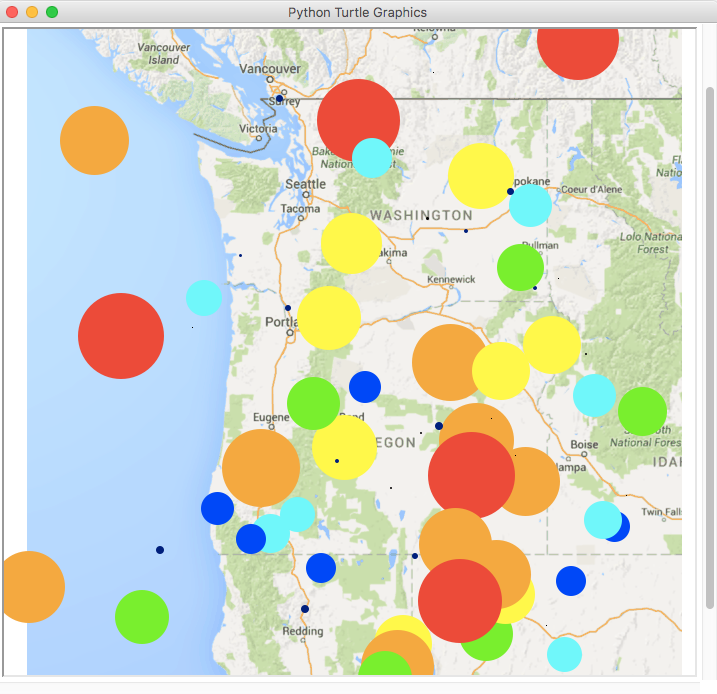
\includegraphics[width=\linewidth]{mags.png}
    \caption{Magnitudes}
  \end{subfigure}
  \begin{subfigure}[b]{0.65\linewidth}
    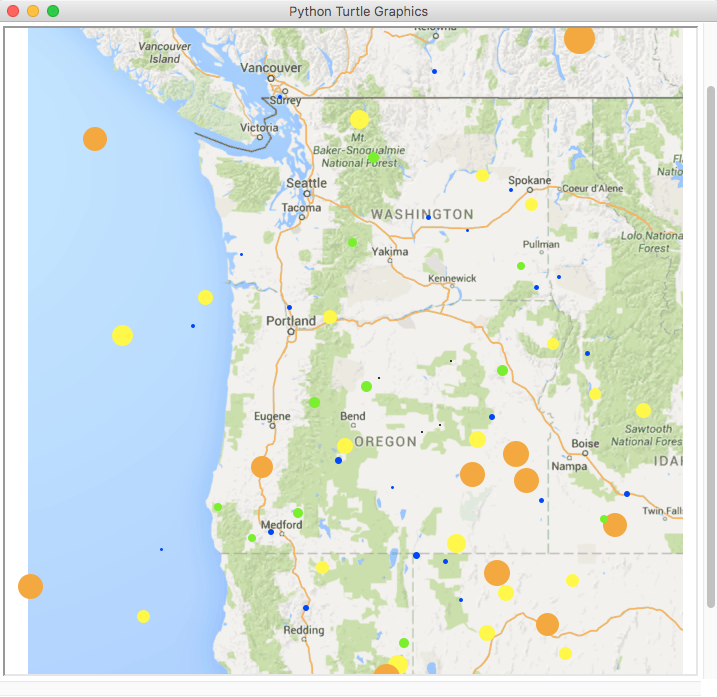
\includegraphics[width=\linewidth]{depths.png}
    \caption{Depths}
  \end{subfigure}
  \caption{Plotting Magnitudes and Depths from the same test case}
  \label{fig:magsdepths}
\end{figure}

The correlation is rather difficult to eyeball but does reflect exactly what is expected. The large red dot due west of Portland has a matching yellow depth dot, which means that a high-intensity quake was fairly deep. The small blue event due west of the Oregon-California border has a matching blue dot in the same place, indicating that a low-intensity quake was not that deep below the surface. One outlier is a sizable orange earthquake covering the Umatilla forest that has a very tiny blue depth dot.

If we consider latitude-longitude oriented north-up, west-left, east-right, south-down, and given the left-slanted-ness of the latitudes and right-slanted-ness of longitudes, we should expect right-leaning longitudes and left-leaning latitudes. This test case should mark the locations of the earthquakes mostly drifting towards the lower-right corner. This is in fact what the program generates (Figure \ref{fig:clusters}).

\begin{figure}[!h]
\centering
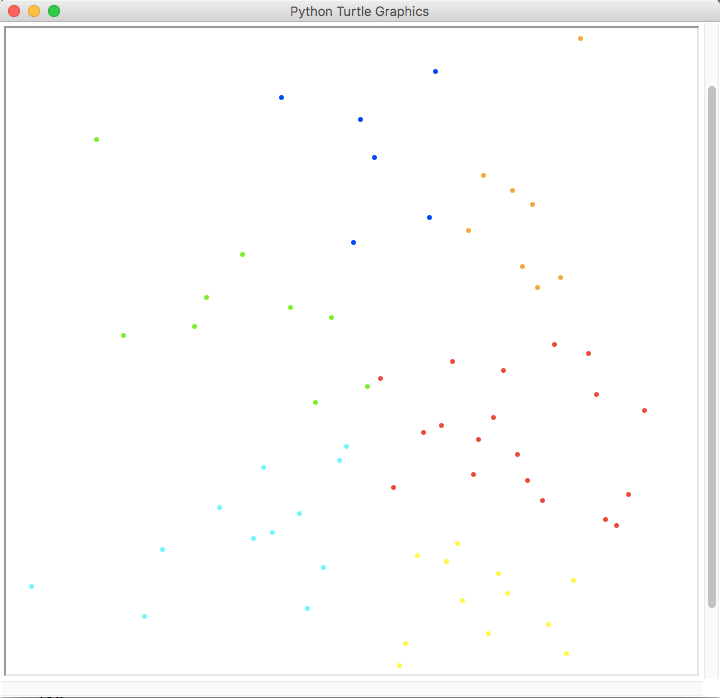
\includegraphics[scale=0.6]{clusters-nobg.png}
\caption{K-Means Clustering of Earthquake events from case 13}
\label{fig:clusters}
\end{figure}